\documentclass[conference]{IEEEtran}
\IEEEoverridecommandlockouts
% The preceding line is only needed to identify funding in the first footnote. If that is unneeded, please comment it out.
\usepackage{cite}
\usepackage{amsmath,amssymb,amsfonts,subcaption}
\usepackage{algorithmic}
\usepackage{graphicx}
\usepackage{textcomp}
\def\BibTeX{{\rm B\kern-.05em{\sc i\kern-.025em b}\kern-.08em
    T\kern-.1667em\lower.7ex\hbox{E}\kern-.125emX}}
\begin{document}

\title{Indoor Localization through Visible Light Characterization using Front-Facing Smartphone Camera
\thanks{}
}
\author{
\IEEEauthorblockN{Charles Carver}
\IEEEauthorblockA{\textit{Dept. of Physics \& Eng. Physics} \\
\textit{Fordham University}\\
Bronx, NY \\
ccarver1@fordham.edu}
\\
\IEEEauthorblockN{Matthew Stafford}
\IEEEauthorblockA{\textit{Dept. of Comput. Sci. \& Eng.} \\
\textit{University of Buffalo}\\
Buffalo, NY \\
mcstaffo@buffalo.edu}
\and
\IEEEauthorblockN{Shela Wu}
\IEEEauthorblockA{\textit{Courant Inst. of Math. Sci.} \\
\textit{New York University}\\
New York, NY \\
shela.wu@nyu.edu}
\\
\IEEEauthorblockN{Dr. N. Sertac Artan}
\IEEEauthorblockA{\textit{Dept. of Elect. \& Comput. Eng.} \\
\textit{New York Institute of Technology}\\
New York, NY \\
nartan@nyit.edu}
\and
\IEEEauthorblockN{Adriana Rogers}
\IEEEauthorblockA{\textit{Dept. of Math. Sci.}\\
\textit{Lewis \& Clark College}\\
Portland, OR \\
rogers.adriana@gmail.com}
\\
\IEEEauthorblockN{Dr. Ziqian Dong}
\IEEEauthorblockA{\textit{Dept. of Elect. \& Comput. Eng.}\\
\textit{New York Institute of Technology}\\
New York, NY \\
ziqian.dong@nyit.edu}
}
\maketitle

\begin{abstract}
Research conducted in the field of localization with passive light, or using the intrinsic properties of light to determine a person's location, has seen increased growth in recent years. Specifically, fluorescent lights have been shown to exhibit distinct frequencies which can be recorded, along with their positions, for future lookup and positioning. Developments have been made in utilizing this phenomenon with a smartphone's high-resolution back-facing camera, however the constant flipping between the camera and the screen results in a poor user experience. In this paper, we propose an algorithm for extracting and analyzing both loop-shaped and tubular fluorescent lights. Similarly, we contribute an improved method for detecting frequency characteristics of unmodified fluorescent lights using a smartphone's front facing camera, therefore eliminating the need to constantly flip the phone.

\end{abstract}

\begin{IEEEkeywords}
visible light localization, indoor positioning system, passive light source, localization with passive light, localization with visible light
\end{IEEEkeywords}

\section{Introduction}\label{section:introduction}

\begin{figure}
\centerline{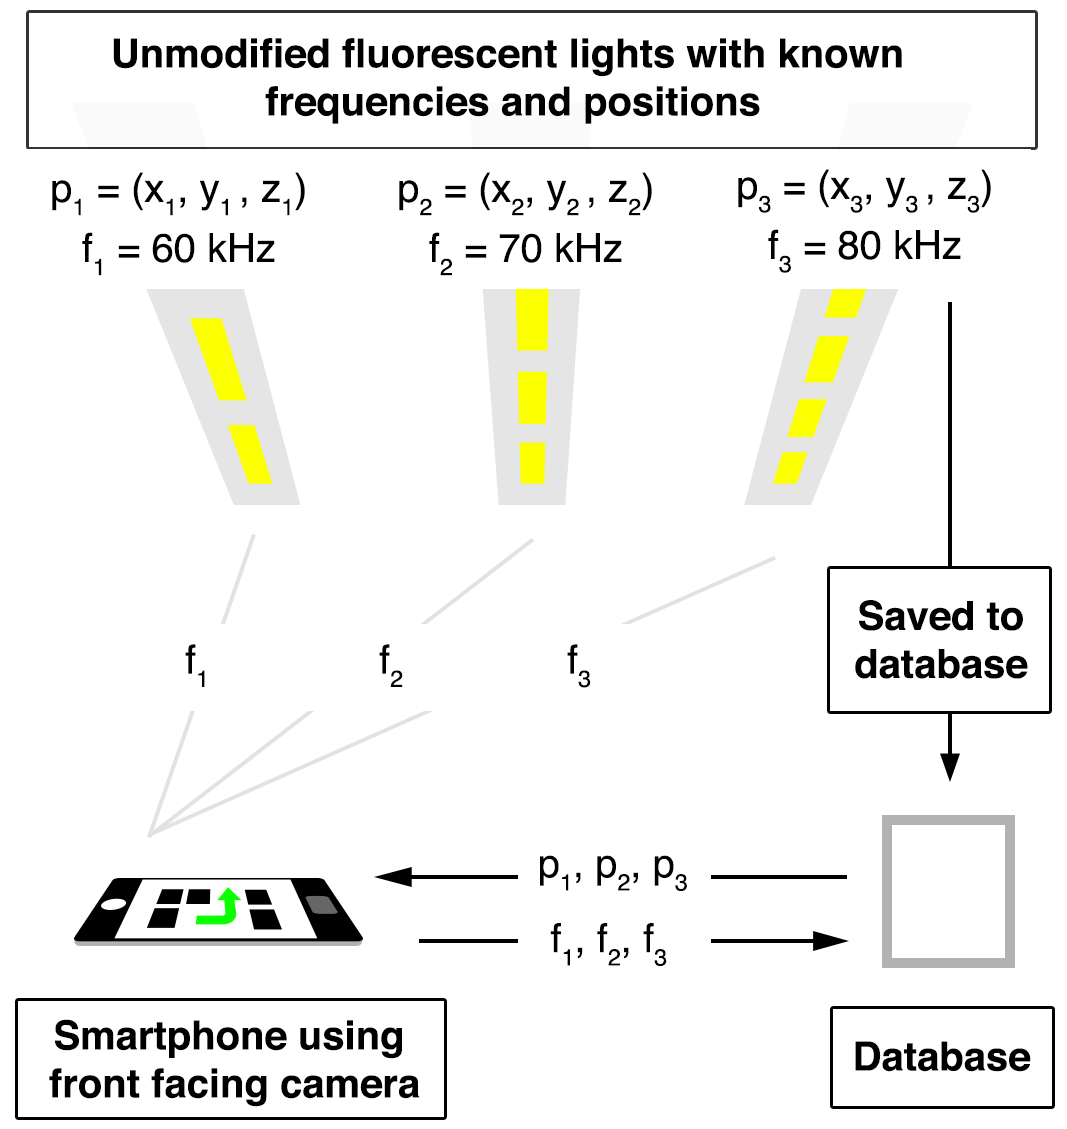
\includegraphics[width=1.0\columnwidth]{figures/concept.jpg}}
	\caption{Concept art showing how known fluorescent light positions and frequencies can be used for indoor localization without infrastructure modifications.}
	\label{fig:poc}
\end{figure}

In this paper, we explore the feasibility of using a standard smartphone's front-facing camera to accurately distinguish between unmodified fluorescent lights. We investigate this hypothesis by processing video frames taken in a controlled environment. We are eventually able to observe unique frequency characteristics with a custom image processing algorithm for both rectangular and looped fluorescent lights.

\subsection{Motivation}

Over the past few years, the prevalence of location based services, such as Global Positioning System (GPS), has risen in parallel with the increased adoption of smartphones. GPS, however, is generally unsuitable for indoor positioning as radio waves do not travel easily through solid objects, e.g., walls. Consequently, when GPS is used within a building, its signals are attenuated and scattered, making it an impractical method for error-less indoor localization.

In an effort to overcome the limitations of GPS, researchers have refocused their attention on developing indoor positioning systems (IPS). These systems utilize numerous types of signals that offer increased location accuracy when used indoors. Research has also been conducted on using existing radio frequency  (RF) systems, such as WiFi and Bluetooth, to refine IPS technology \cite{do2016depth}. While the accuracy of WiFi-based indoor positioning systems are greater than GPS-based systems, they still encounter interference and security issues characteristic of radio wave communication.

Recently, visible light localization (VLL) systems have become prominent areas of research due to their high security and minimal interference qualities. These qualities can be attributed to the line of sight (LoS) characteristic that visible light exhibits, i.e., successful data transmission is only guaranteed if the receiver is within the field of vision of the transmitter. Contrary to how WiFi-based indoor positioning systems utilize an existing wireless infrastructure, most VLL systems require purposefully built light sources that are installed overhead. Consequently, the costs incurred by retrofitting existing infrastructures make these systems cumbersome and difficult to adopt.

Fluorescent lights, however, have become an attractive candidate for VLL transmitters as they require no modifications to be used within a VLL system. Due to how fluorescent lights operate, each light flickers at a unique characteristic frequency (CF) that is imperceptible to the human eye. This CF is recognized as the dominant frequency of the fluorescent light's waveform. One recent work introduces a VLL system named ``LiTell'' that utilizes unmodified fluorescent lights and a commercial smartphone \cite{zhang2016litell}. LiTell's setup initially requires a database of fluorescent light locations and their corresponding CFs. A smartphone then captures RAW images of any overhead fluorescent lights using the phone's back-facing camera. Image processing is then applied to the captured images, extracting the fluorescent light's aliased frequency (a value dependent on the light's CF and the camera's sampling rate). After performing simple arithmetic, the CF is then extracted and matched to the previously built database. Finally, using straightforward geometry, the smartphone's exact location is computed with a 90.3\% accuracy.

The biggest drawback of LiTell's system is its reliance on a smartphone's back-facing camera. Although the back-facing camera is capable of capturing high resolution, RAW images, it requires the user to flip his or her phone around while using the localization application. Given the recent improvements in front-facing camera quality, however, we believe that there is room for development in this area with respect to localization. Using the front-facing camera for CF-based VLL is an intuitive improvement as it improves the user experience and creates a more streamlined, easily adoptable VLL system. This research, therefore, begins by hypothesizing that by using a smartphone's front-facing camera, we can sufficiently identify the characteristic frequency of a fluorescent light which may then be used for secure, indoor localization. We attempt this by examining a short video, taken by a smartphone's front-facing camera, to sample the frequency of any overhead lights. We then implement a video processing algorithm to identify the CF of both standard long-shaped and loop-shaped fluorescent lights by analyzing many frames within the video.

\subsection{Organization}

Section \ref{section:relatedworks} begins by discussing existing VLL systems and comparing them. Required concepts are explained in Section \ref{section:technicalbackground}, including a background on how fluorescent lights and smartphone cameras operate. Our experimental setup and image processing algorithm are explained in Section \ref{section:experimentalsetup}. We analyze our results in Section \ref{section:results}. We propose suggestions for future improvements in Section \ref{section:futurework}.

\section{Related Works}\label{section:relatedworks}

\subsection{Visible Light Localization}

Utilizing visible light for indoor localization is a growing area of research as visible light provides a secure alternative to traditional RF-based systems. Due to the vastness of this field, we initially explored a variety of visible light systems and narrowed our research to using visible light for localization purposes. Many forms of VLL build upon existing visible light communication (VLC) schemes that allow for data transmission between LEDs and image sensors/photodiodes. These systems rely on modulating the transmitting LED, essentially turning it on and off at a rate that is imperceptible to the human eye. Then, on the receiving side, the signal is demodulated to retrieve the transmitted data. VLC systems with this basic design can also be used for positioning through means such as: proximity, fingerprinting, triangulation, and vision analysis \cite{do2016depth}. These systems use features such as Received Signal Strength (RSS), Angle of Arrival (AoA), Time of Arrival (ToA), and Time Distance of Arrival (TDoA) to estimate the receiver's distance relative to the observed lights. 

In \cite{kuo2014luxapose}, Luxapose determined a smartphone's location with decimeter-level accuracy by modulating overhead LEDs and using an unmodified smartphone camera. Similarly, \cite{li2014epsilon} focused on improving accuracy in a similar LED-to-smartphone localization setup. These aforementioned examples are considered active VLL systems as the LED is intentionally modulated to send specific data.

\subsection{Passive Source Systems}

Recently proposed passive VLL systems are a promising alternative to active VLL systems \cite{wang2017passive}. Although active VLL systems incur implementation costs, passive VLL systems do not as the light infrastructure remains unmodified. This is because passive VLL systems employ unaltered light sources, such as fluorescent lights or the sun, as location identifiers \cite{wang2017passive}.  For this reason, ample research has been conducted in implementing wide-scale, passive VLL systems \cite{zhang2016litell}\cite{wang2016passive}. Notably, LiTell, an indoor VLL system, uses a mobile application to identify fluorescent lights with a smartphone's back-facing camera \cite{zhang2016litell}.

We investigate the usability of a smartphone's front-facing camera in a passive VLL system. Since the front-facing camera is capable of capturing JPEG images and videos, we test if frequencies can be extracted from either. Similarly, we assess various set-ups and smartphones to obtain the highest signal-to-noise ratio (SNR). In Section \ref{section:compression}, JPEG images are shown to be inoperative in passive VLL settings so we instead focus on using video for accurate CF detection.

\section{Technical Background}\label{section:technicalbackground}

This section explains the concepts integral to understanding localization using a smartphone and fluorescent lights.

\subsection{Fluorescent Lights}

The electric utility industry is essential due to the continuous growth within other fields that require the constant consumption of electrical power \cite{sasaki1994impact}. Energy-efficient devices are generally favored, a particular reason why fluorescent lights are still used within indoor office and retail settings. While incandescent light bulbs generate approximately 15 lumens per watt, a fluorescent bulb can produce 50 to 100 lumens per watt, making them between 4 and 6 times more efficient with less heat produced \cite{lumensperwattcomparison}.

Thus, due to their high level of light output accompanied with a low cost per lumen, fluorescent lights are an accessible source to be used within a VLL system. As explained in Section \ref{section:introduction}, passive VLL systems can use the characteristic frequencies of fluorescent lights as unique transmitters. As defined by LiTell, the characteristic frequency is a fluorescent light's dominant frequency which occurs at a range twice that of the fundamental frequency \cite{zhang2016litell}. Fluorescent lights were found to flicker at a CF greater than 80 kHz which is imperceptible to the human eye. This CF is the result of the manufacturing process which results in unavoidable variations in resonant frequencies. LiTell tested 500 fluorescent lights in an office building and found that less than 0.1\% of lights had a difference in frequency less than 10 Hz \cite{zhang2016litell}. Fluorescent lights, therefore, can be adequately distinguished from one another and are thus viable transmitters for indoor localization. It's worth noting that fluorescent lights require some time for their CF to stabilize, specifically around 40 minutes. Although this might be an issue in certain settings where lights turn off automatically to conserve power, many locations, e.g. supermarkets, keep their lights on for the entire day thus ensuring FL stability.

\subsection{Smartphones Cameras}

VLL systems that are compatible with mobile devices are desirable as they can be easily utilized by anyone with a smartphone. VLL systems that use photodiodes or other light sensors, however, incur the cost of custom receivers which  detract from widespread utilization. For example, in \cite{xu2016indoor}, a VLL system is developed using an LED light and at least 3 photodiodes to accurately determine location. While such a system achieves centimeter level accuracy, it cannot be easily implemented on a large scale. Our research utilizes a conventional smartphone's front-facing camera to take a short video of any overhead fluorescent lights. This video is then processed and the CF is determined.

\subsection{Rolling Shutter Effect}

\begin{figure}[!ht]
\centerline{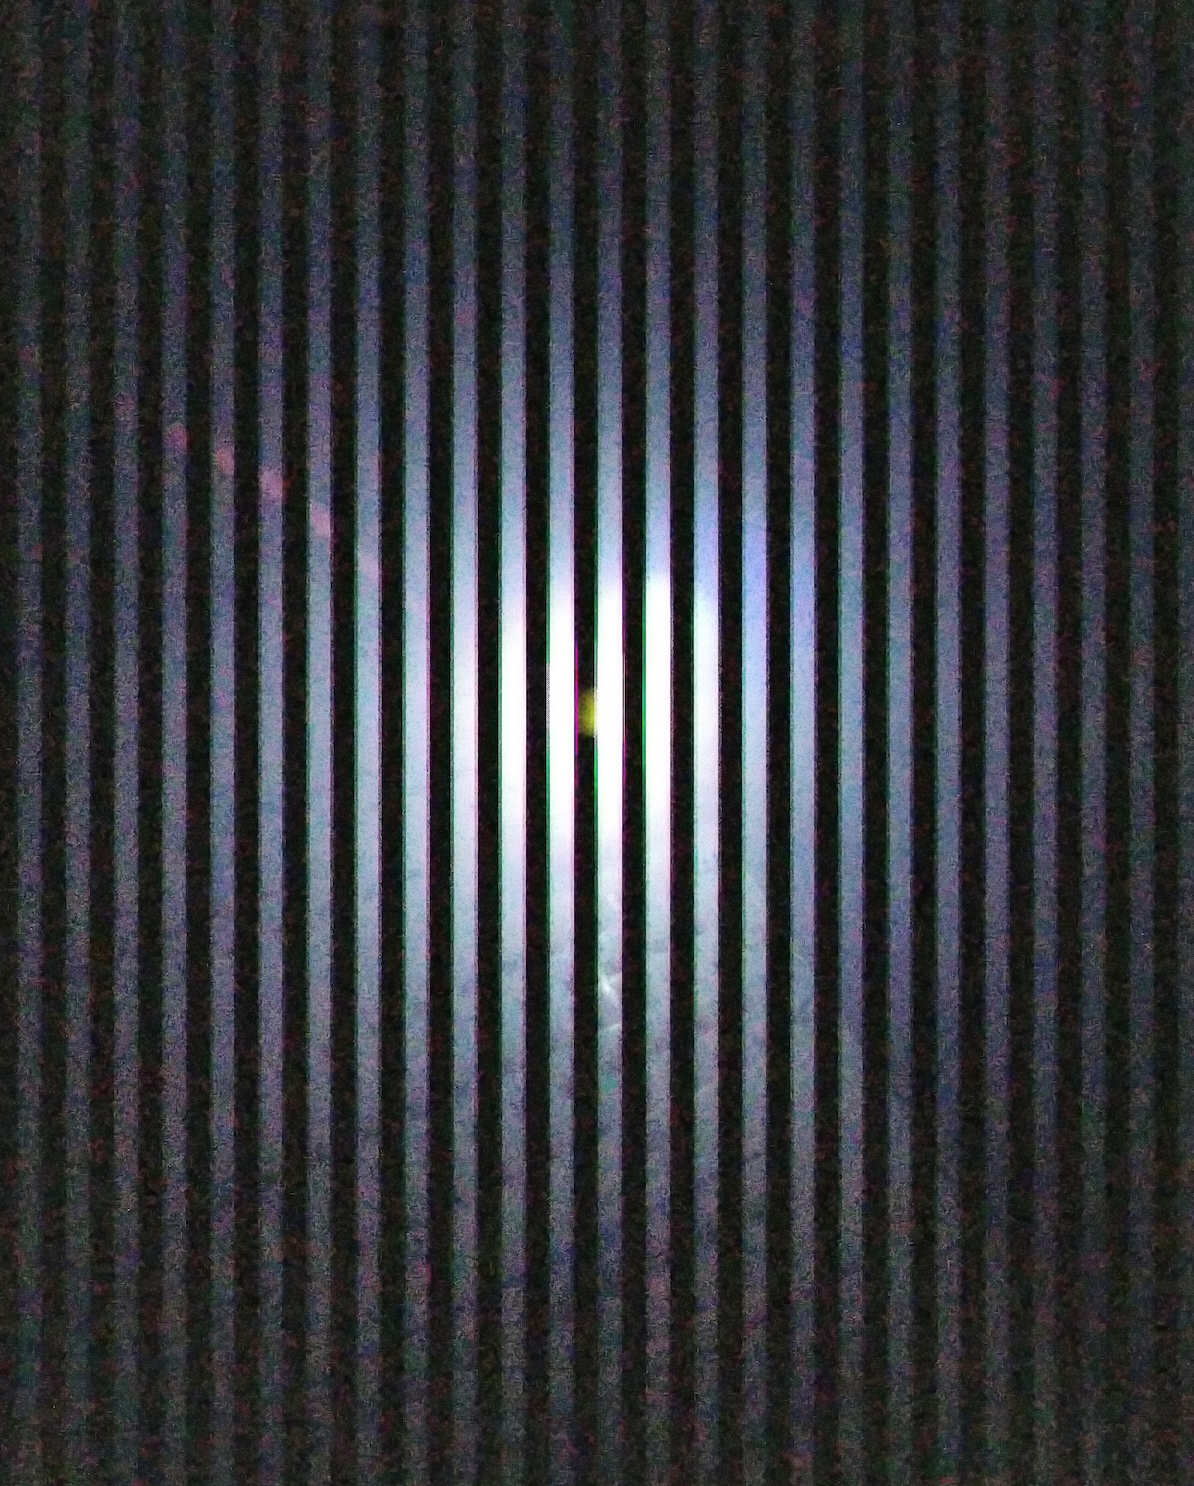
\includegraphics[width=0.5\columnwidth]{figures/rolling_shutter.jpg}}
	\caption{The rolling shutter effect captured by a Samsung Galaxy S8 over a modulated LED.}
	\label{fig:rollingshutter}
\end{figure}

We are able to use a smartphone's camera to sample high frequencies due to the rolling shutter effect. Most smartphone cameras use CMOS image sensors which sequentially expose sets of light sensors resulting in a banding effect as shown in Fig. \ref{fig:rollingshutter} \cite{liang2008analysis}. If the smartphone is held in portrait mode, so the length of the fluorescent light aligns with the width of the screen, then the bands will run across the phone from left to right. The rate at which one column of the image is exposed is called the sampling rate, which is theoretically calculated according to $W \times fps$, where $W$ is the width of the image in pixels. The width of these bands will vary depending on the modulation frequency which can be calculated through image processing techniques as explained in Section \ref{section:imageprocessing}.

If the camera's sampling rate is faster than the frequency, the camera is able to detect at least one period of modulation. An issue that arises with fluorescent lights, however, is that their CF is much faster than the sampling rate of typical smartphone cameras. Specifically, \cite{zhang2016litell} found that most FLs have CFs between 40 kHz and 200 kHz. This, intuitively, means that the smartphone observes an aliased frequency instead of the desired CF. Aliasing is an effect that occurs when the sampling rate is too slow to acquire the original signal. Specifically, aliasing occurs when a signal with frequency $f$ is not sampled at at least $2f$, i.e., the Nyquist frequency. This causes the frequency of the signal to be folded back, resulting in a false mirror image of the signal at frequencies below $f$ \cite{cerna2000fundamentals}. To find the aliased frequency, we convert a time domain signal of the fluorescent light to the frequency domain by applying a fast Fourier transform (FFT). We then define our estimate of the true CF, $f_e$, as: 
\begin{equation}
f_e = N f_s \pm f_a
\end{equation}
where $N$ is an integer greater than or equal to $0$, $f_s$ is the sampling frequency of the smartphone, and $f_a$ is the aliased frequency \cite{zhang2016litell}.

\subsection{Camera Settings}

When taking short videos of the light, we alter the default camera settings to optimally sample the lights and boost SNR. The main settings that we alter are the shutter speed, ISO, focus, and resolution. Shutter speed, or exposure time, is the length of time that the shutter allows in light. To detect fast frequencies, this value is minimized. 

ISO is a measure of the sensitivity of the image sensors to light. A lower ISO means the camera is less sensitive to light so only the brightest light sources are captured, essentially resulting in less visible grain. In \cite{zhang2016litell}, it is recommended that the ISO be maximized to increase the signal to noise ratio (SNR), however we found that at the maximum ISO level, the image became oversaturated. This discrepancy is due to our smartphone having a slower shutter speed than the Nexus 5 used in \cite{zhang2016litell}, meaning our smartphone captured more light over a greater period causing oversaturation.

In many conventional settings, fluorescent lights are covered by filters, as shown in Fig. \ref{fig:lighttypes}., that disperse their light across a larger area. These filters, however, generally have distinct lattice structures that skew the image. Consequently, the video is blurred to mitigate the spatial artifacts that would ultimately affect CF identification. 

Finally, we use the highest possible video resolution as this maximized the sampling rate of our camera. 

\subsection{Compression Methods}\label{section:compression}

Previous works that use image processing to distinguish modulation frequencies use the back-facing camera to take RAW photos. Utilizing RAW images allows for a more accurate view of the light and improves CF distinguishability during the image processing stage \cite{zhang2016litell}. To increase usability, we utilize the front-facing camera. Modern smartphones do not take RAW images with the front-facing camera and only take compressed JPEGs and videos. JPEGs utilize a compression method that removes high intensity frequencies that would normally not be visible to the human eye \cite{wallace1992jpeg}. MP4s, however, are not compressed in the same fashion and are thus an alternative when using the front-facing camera.

\section{Experimental Setup}\label{section:experimentalsetup}

\begin{figure}
\centerline{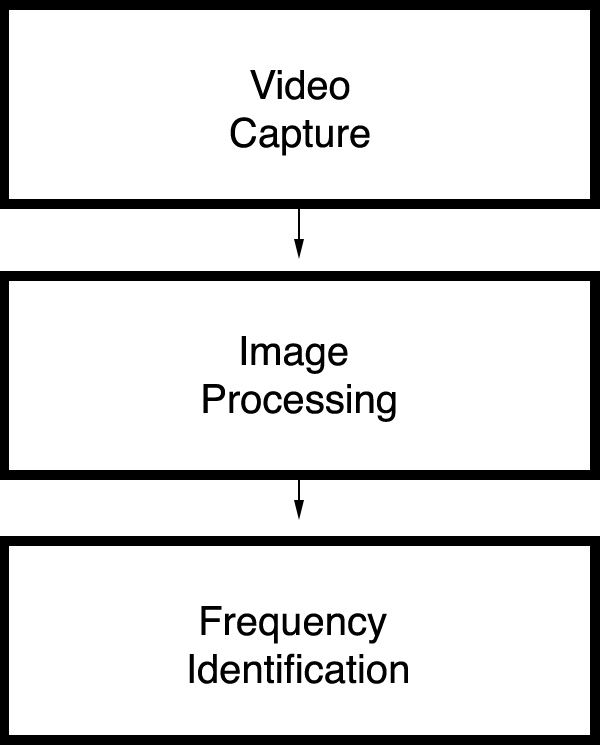
\includegraphics[width=0.5\columnwidth]{figures/block.jpg}}
	\caption{A block diagram of our experiment.}
	\label{fig:block}
\end{figure}

Our experimental setup is represented by Fig. \ref{fig:block} and is broken up into three steps: video capture, image processing, and frequency identification.

\subsection{Video Capture}
\subsubsection{Camera Specifications}

\begin{table}
	\caption{Phone resolution comparison}\label{table:resolution}
	\begin{center}
	\begin{tabular}{|l|l|}
	\hline
	Phone Type        & Resolution  \\ \hline
	Samsung Galaxy S8 & 2880 x 2160 \\ \hline
	Samsung Galaxy S7 & 2592 x 1944 \\ \hline
	Google Nexus 5    & 1280 x 960  \\ \hline
	\end{tabular}
	\end{center}
\end{table}

\begin{figure}
\centerline{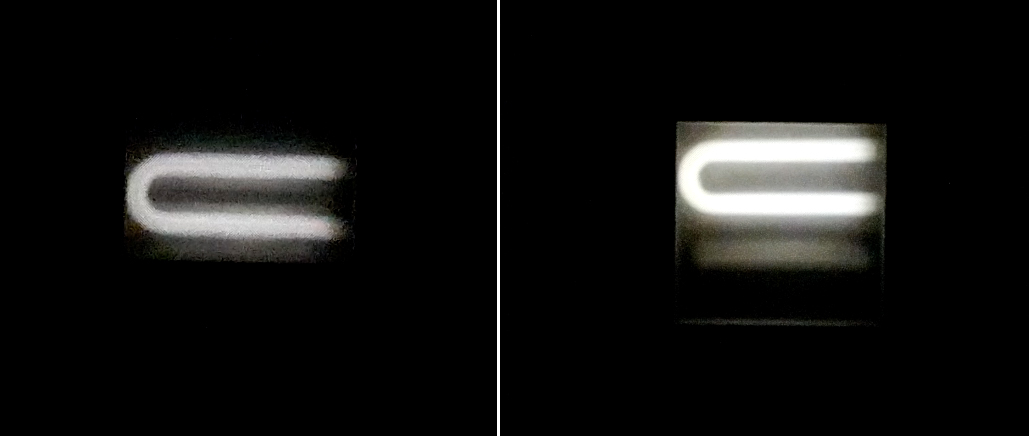
\includegraphics[width=0.9\columnwidth]{figures/s7_vs_s8.jpg}}
	\caption{Image quality of the Samsung S7, left, vs. the Samsung S8, right.}
	\label{fig:s7_vs_s8}
\end{figure}

We use Open Camera, an open source camera application, that allows for alteration of features such as ISO sensitivity, shutter rate, and video resolution. Initially, we tested three different phones: the Google Nexus 5, the Samsung Galaxy S7, and the Samsung Galaxy S8 (see Table \ref{table:resolution}). Out of all of these, the Samsung Galaxy S8 was the most suitable candidate given its higher resolution front-facing camera and support for the camera2 Android API. The difference in image quality can be visibly seen in Fig. \ref{fig:s7_vs_s8}. Certain camera settings are held constant throughout testing, including the shutter speed (1/14388.7s) and the video resolution (2880 x 2160). We create a ``forced macro mode'' that is implemented via the ``Focus Locked'' mode: by locking the focus on an object that is within a 5 cm proximity to the camera, we are able to create an effective blur to counteract the effects of the patterned light filter.

\subsubsection{Testing Set-up}\label{section:testingsetup}

\begin{figure}
\centerline{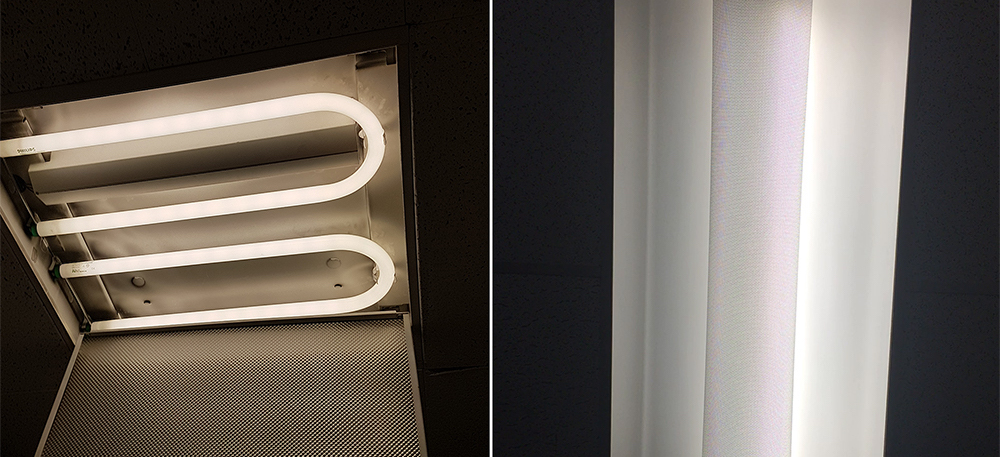
\includegraphics[width=0.9\columnwidth]{figures/comparison.jpg}}
	\caption{Two types of common light shapes, looped (left) and tube (right).}
	\label{fig:lighttypes}
\end{figure}

\begin{figure}
\centerline{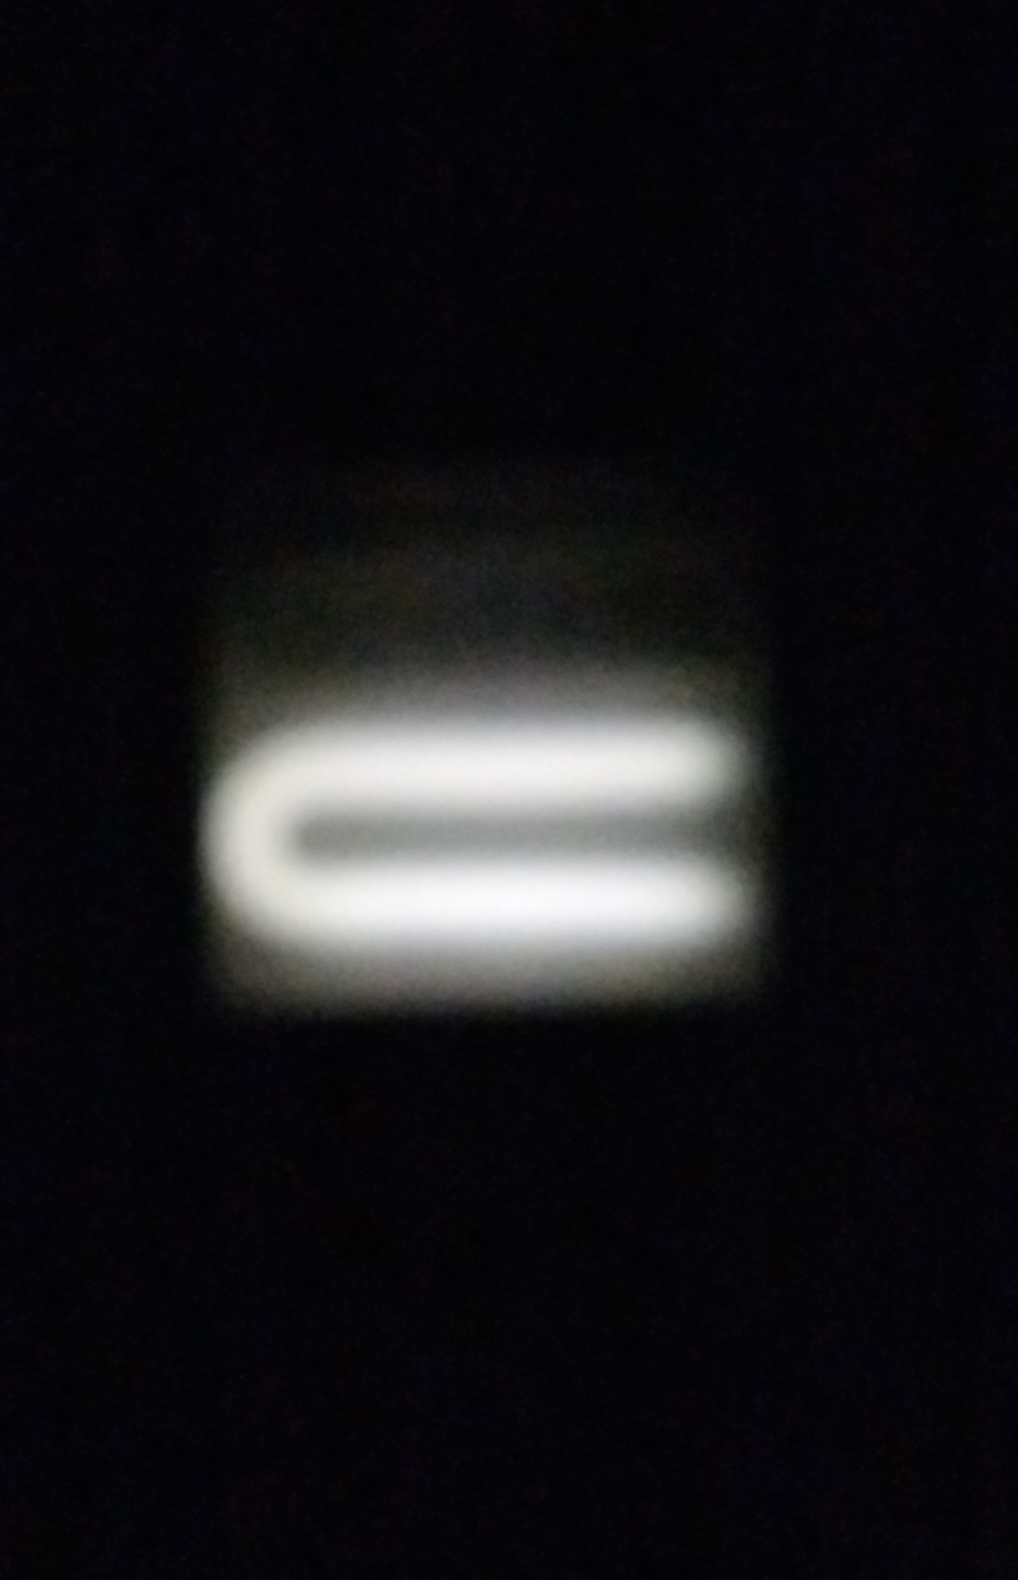
\includegraphics[width=0.5\columnwidth]{figures/looped.jpg}}
	\caption{The optimal orientation for data collection, with the long side of the light occupying the short side of the captured image.}
	\label{fig:loopedlight}
\end{figure}

To evaluate the viability and performance of using the front-facing camera to detect high frequencies, we construct a controlled environment consisting of two differently shaped fluorescent lights: a pair of looped lights and a single straight light as shown in Fig. \ref{fig:lighttypes}. Each light is turned on individually and all ambient light is excluded from the environment. Prior to testing, each light is left on for at least 40 minutes to ensure frequency stability. A tripod is placed directly underneath the fluorescent lights and set to its tallest height, approximately 143 cm tall. Thus, in an approximately 2.74 m high room, the smartphone camera lays about 131 cm away from the fluorescent light filters. The smartphone is oriented in portrait mode so that the long edge of the fluorescent light fits within the short edge of the camera's field of vision as shown in Fig. \ref{fig:loopedlight}.

Once the camera is calibrated to the proper settings, data collection begins at ISO levels of approximately 800, 1200, 1600, and 2400. 90 second videos are recorded at each ISO level to ensure at least 60 seconds of usable data.

\subsection{Image Processing }\label{section:imageprocessing}

\begin{figure*}
	\begin{center}
	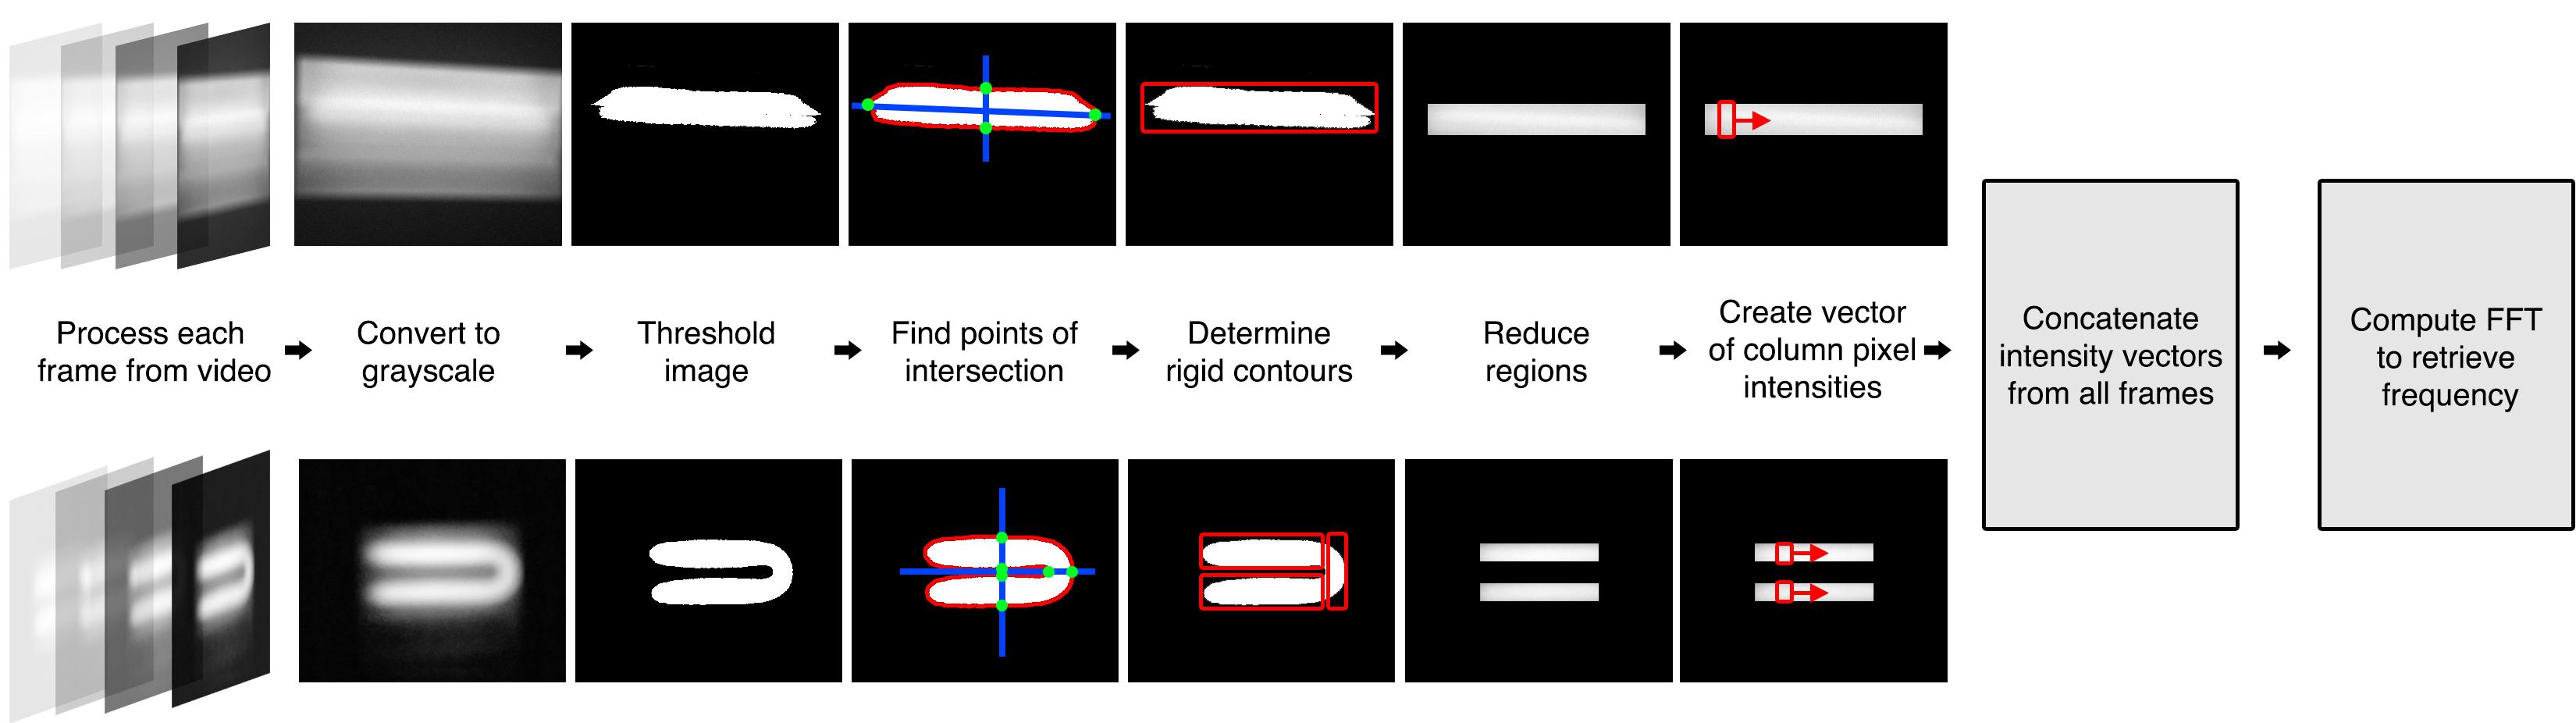
\includegraphics[width=1\textwidth]{figures/diagram.jpg}
	 \caption{Image processing algorithm for isolating regions of light.}\label{fig:diagram}
	 \end{center}
\end{figure*}

The image processing algorithm implements many of the same functions described by \cite{zhang2016litell} but entirely in MATLAB. This process is explained graphically in Fig. \ref{fig:diagram}. 

To begin, a starting frame index and end frame index are specified. To ensure the banding effect is in the correct direction, the image is flipped to portrait mode. The image is converted to grayscale and scaled to a significantly smaller size for speed improvements. From there, the image is thresholded to isolate the most intense region of light. Morphological opening and closing is then performed to remove any small pixel groupings and connect the remaining regions. Next, boundaries are found across the image and the area of each region is computed. The largest boundary is considered the main portion of  light and all other boundaries are discarded.

Now that the light has been effectively isolated, a rigid contour is drawn around the shape. Since fluorescent lights are often not single rectangular tubes, but instead irregular shapes, we wanted to allow for the possibility of CF detection over varying light shapes. Given our experimental conditions, we build in the functionality to analyze looped lights as shown in Fig. \ref{fig:loopedlight}. The midpoint is found on both the x-axis and y-axis, effectively bisecting the light in both dimensions. The points at which the boundary intersects these lines dictate the shape of the light. When four indices are found, the FL is considered looped whereas two indices indicate a single rectangular FL. The individual components are then extracted from the original image and pushed to an array for processing.

To process each shape, the individual components are then converted back to grayscale. Each column of the component is looped over, summing the intensity and pushing it to an array. The resulting intensity vector is fit to a 6th degree polynomial to remove lens vignetting \cite{zhang2016litell}. One departure from \cite{zhang2016litell} is the omission of deinterleaving as the images are already compressed. Finally, the intensities are added to an array containing the intensities from previous frames.

\subsection{Frequency Identification}\label{section:frequencyidentification}

Finally, to determine the aliased CF of the light, a fast Fourier transform is applied to the vector of intensities. The number of samples for the signal is the size of the intensity vector.

The sampling frequency of the smartphone camera is calculated by multiplying the video's frame rate by the video's smaller dimension. For the Samsung Galaxy S8 with a video resolution of $2880 \times 2160$ and a framerate of $30$, the estimated sampling frequency is $2160 \times 30 = 64.8$ ksps. However, error in the sampling frequency amplifies the error in the calculated CF. It is important, therefore, to find the precise sampling frequency of the camera. To do this, we take a video of a modulated LED using the same camera settings as outlined in Section \ref{section:testingsetup}. We use a function generator to power the LED at a range of frequencies (under 5 kHz) and sample the resulting banding effect of a random frame. At each frequency, the width of these bands differ. We then apply image processing, as explained in Section \ref{section:imageprocessing}, to determine the average width of each black and white band at each frequency tested. Next, we reconstruct the original signal but with the averaged width for each alternating band. Then, we run a fast Fourier transform over the new vector and guess and check the input sampling frequency until the FFT results in a peak frequency at the modulation frequency. For our experiment, the actual sampling frequency found over several trials is $64.93$ ksps.

We then analyze the raw FFT output (to preserve all subtle frequency components) and look for any outlier frequencies that peak within the noisy signal. Windowing the Fourier transformation accentuates prominent peaks but occasionally diminishes unique frequency components that we are interested in observing.

\section{Results}\label{section:results}

\subsection{Image Processing}

\begin{figure*}[!h]
	\begin{subfigure}{.245\textwidth}
		\centering
		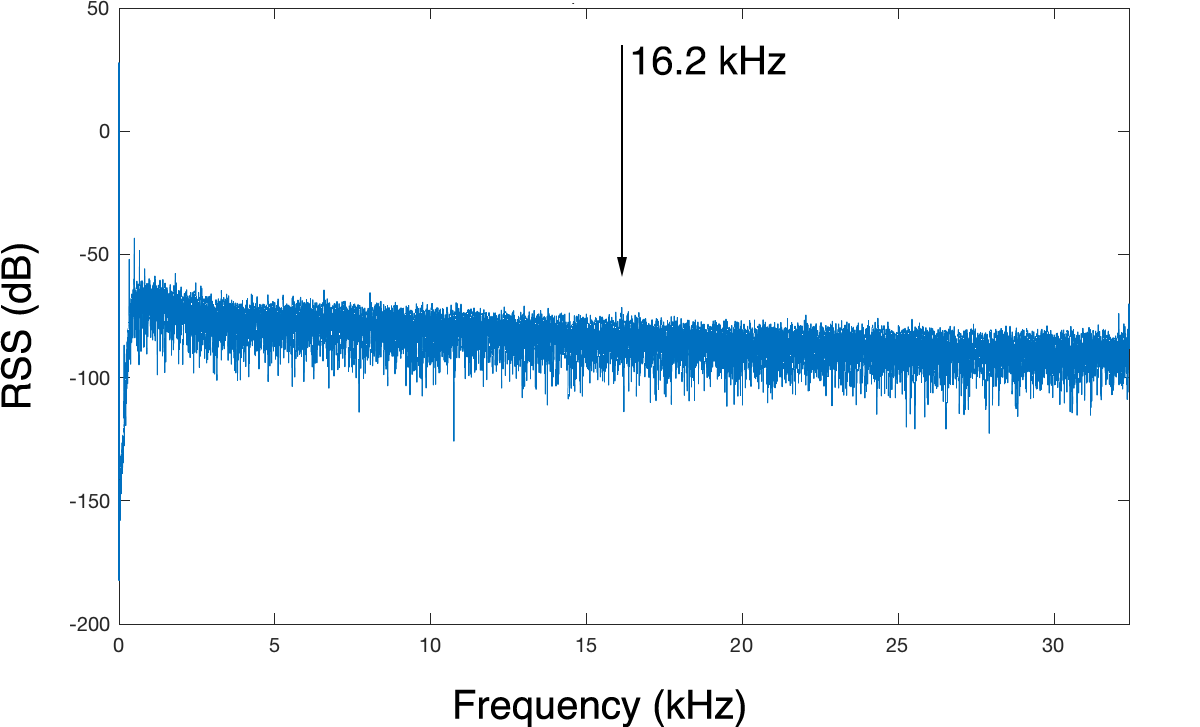
\includegraphics[width=1\linewidth]{figures/A/light_1_16_2.png}
		\caption{Light \#1}
	\end{subfigure}
	\begin{subfigure}{.245\textwidth}
		\centering
		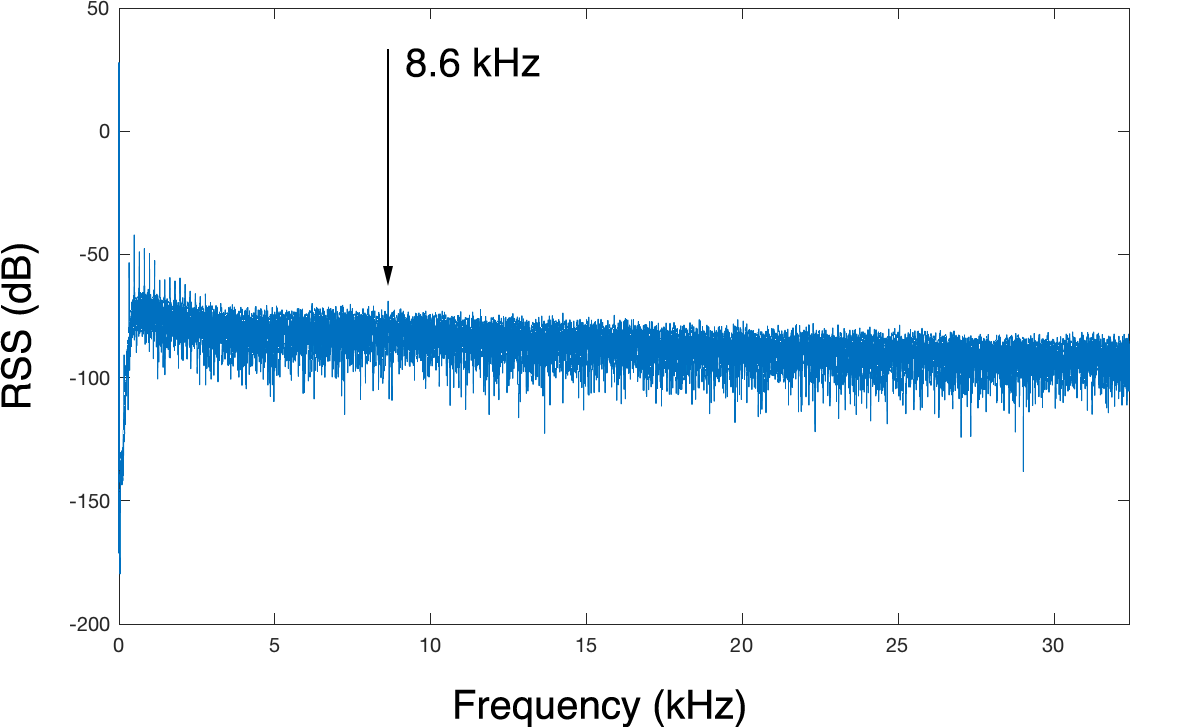
\includegraphics[width=1\linewidth]{figures/A/light_2_8_6_video.png}
		\caption{Light \#2}
	\end{subfigure}
	\begin{subfigure}{.245\textwidth}
		\centering
		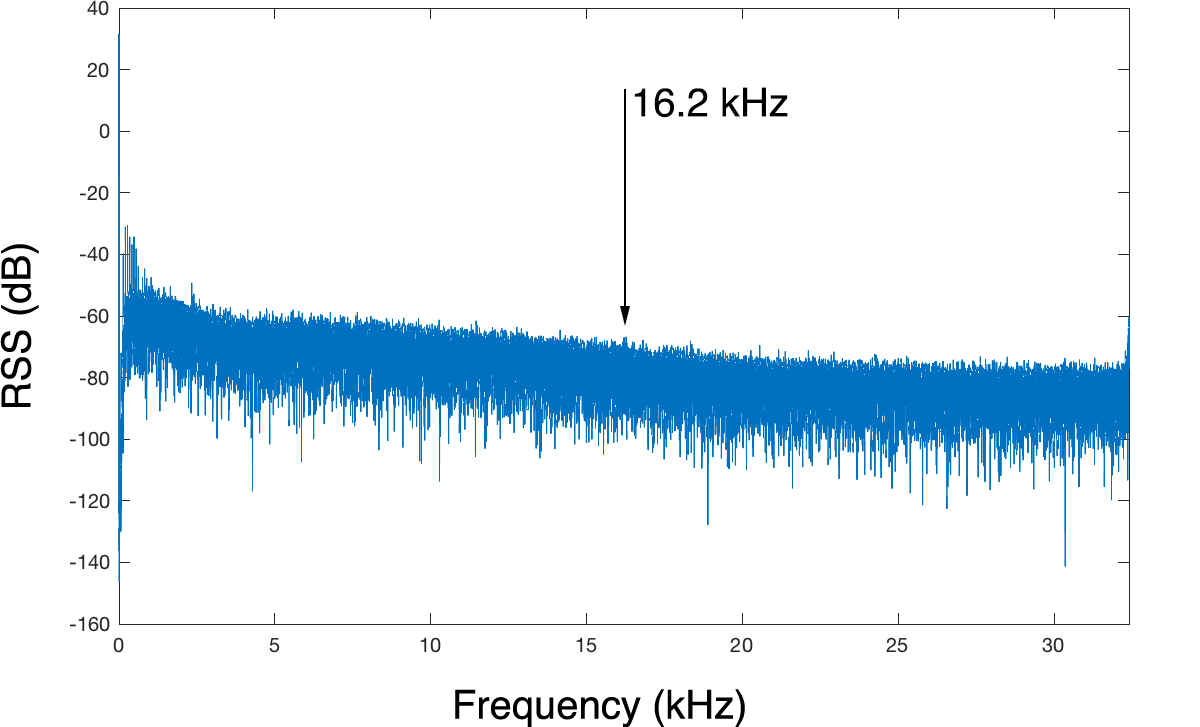
\includegraphics[width=1\linewidth]{figures/A/light_3_16_2.png}
		\caption{Light \#3}
	\end{subfigure}
	\begin{subfigure}{.245\textwidth}
		\centering
		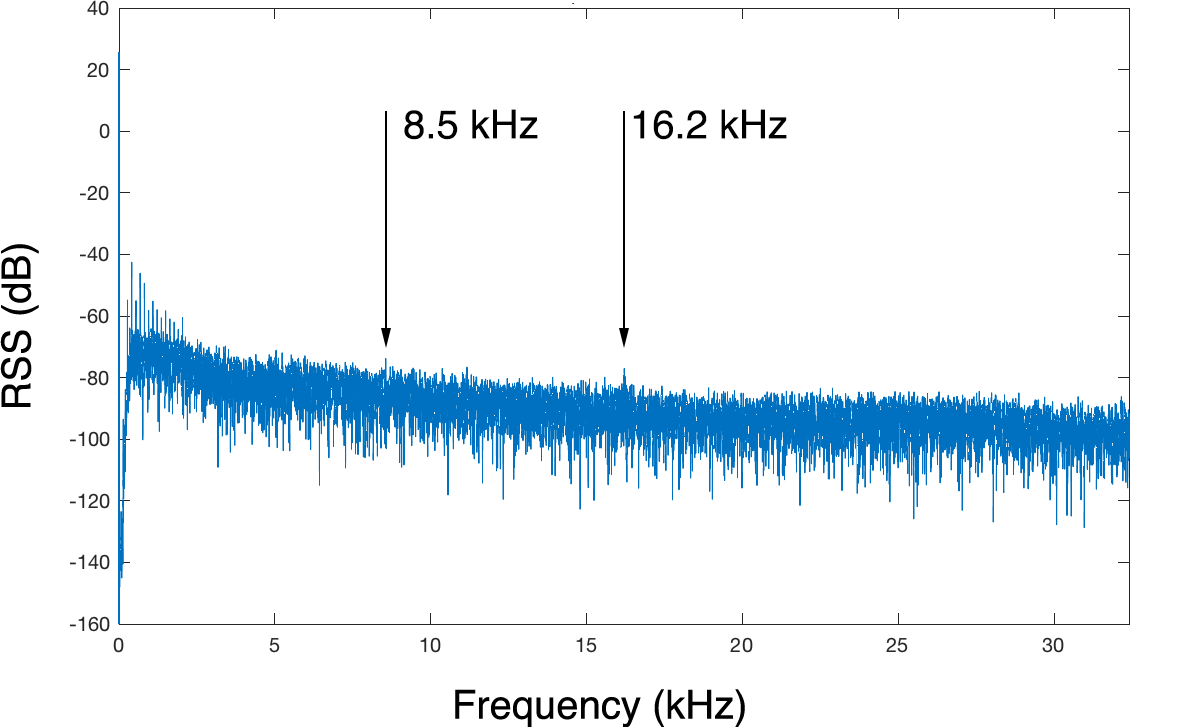
\includegraphics[width=1\linewidth]{figures/B/light_2_8_6_16_2_jpegs.png}
		\caption{Light \#3 after JPEG analysis}
		\label{fig:frequencydistortions_jpeg}
	\end{subfigure}
	\caption{Frequency distortions found across three different lights.}
	\label{fig:frequencydistortions}
\end{figure*}

To evaluate our image processing algorithm, we analyze the frequency data output by the FFT over various ISO levels for each light. After analyzing the resulting peaks in the data, we find that there are consistent peaks across all three lights with various levels of intensity. As shown in Fig. \ref{fig:frequencydistortions}., we can see that across the three lights, the RSS peaks at around 8.6 kHz and 16.2 kHz. The spectrum in Fig. \ref{fig:frequencydistortions_jpeg}. was calculated from JPEG images and shows peaks at both 8.5 and 16.2 kHz in the same dataset. Since these frequencies are found within all three datasets, they are either erroneous side effects of our image processing algorithm/MP4 compression or simply frequencies common to all FLs.

\begin{figure*}[!h]
	\begin{subfigure}{.33\textwidth}
		\centering
		
\includegraphics[width=1\linewidth]{figures/C/801.png}
		\caption{ISO 801}
	\end{subfigure}
	\begin{subfigure}{.33\textwidth}
		\centering
		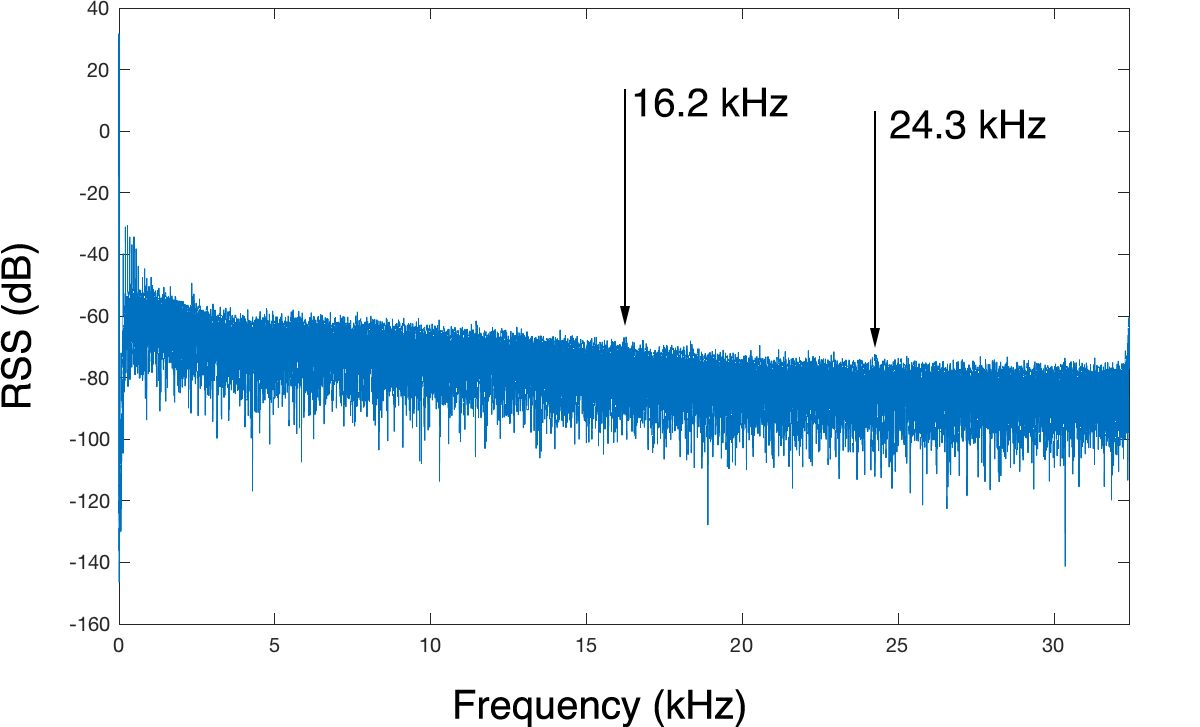
\includegraphics[width=1\linewidth]{figures/C/1196.png}
		\caption{ISO 1196}
	\end{subfigure}
	\begin{subfigure}{.33\textwidth}
		\centering
		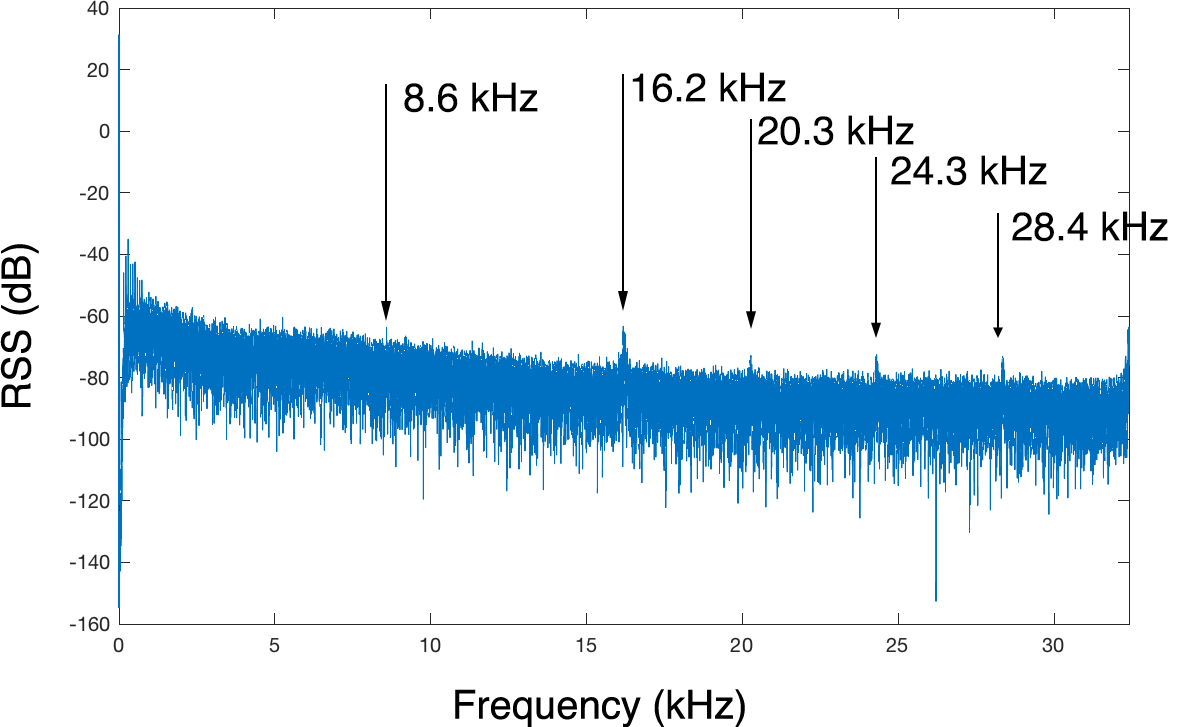
\includegraphics[width=1\linewidth]{figures/C/2401.png}
		\caption{ISO 2401}
	\end{subfigure}
	\caption{ISO's effects on frequency distortions for light \#3.}
	\label{fig:isosimpact}
\end{figure*}

\begin{figure*}[!h]
	\begin{subfigure}{.33\textwidth}
		\centering
		
\includegraphics[width=1\linewidth]{figures/D/801.png}
		\caption{ISO 801}
	\end{subfigure}
	\begin{subfigure}{.33\textwidth}
		\centering
		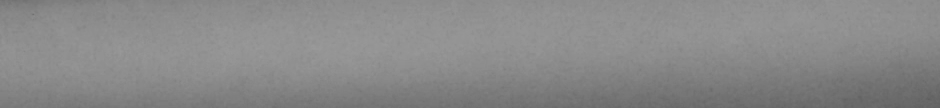
\includegraphics[width=1\linewidth]{figures/D/1196.png}
		\caption{ISO 1196}
	\end{subfigure}
	\begin{subfigure}{.33\textwidth}
		\centering
		
\includegraphics[width=1\linewidth]{figures/D/2401.png}
		\caption{ISO 2401}
	\end{subfigure}
	\caption{Isolated regions of light at varying ISO levels for light \#3.}
	\label{fig:isosexamples}
\end{figure*}

Similarly, we evaluate how these peaks appear at varying ISO levels. Fig. \ref{fig:isosimpact}. shows the dominant frequencies at ISO values of 801, 1196, and 2401 for one single light. Samples from each of these ISO levels are shown in Fig. \ref{fig:isosexamples}. A peak at 16.2 kHz is consistent among all three ISO levels, with the highest ISO level exaggerating consecutive peaks spaced roughly in increments of 4 kHz (potentially representing harmonic frequencies).

Given these results, it appears that a higher ISO value skews the image processing and accentuates common frequencies while dampening unique frequencies. This is possibly due to how the image processing algorithm sums across the image's columns and adds up the pixel values. If the camera has a higher ISO value, the resulting image appears more saturated and only the fringes of the light are not completely white. Consequently, the minute differences caused by the FL's flickering are not picked up in a consistent manner and the entire region is simply regarded as white. If the ISO value is lower, however, the small differences between dark and light bands are captured in the grayscale image and not simply washed out. Given our results, we find the optimal ISO setting to be between 800 and 1200 with our given shutter speed and sampling rate.

\subsection{Data Formats}

\begin{figure*}[!h]
	\begin{subfigure}{.5\textwidth}
		\centering
		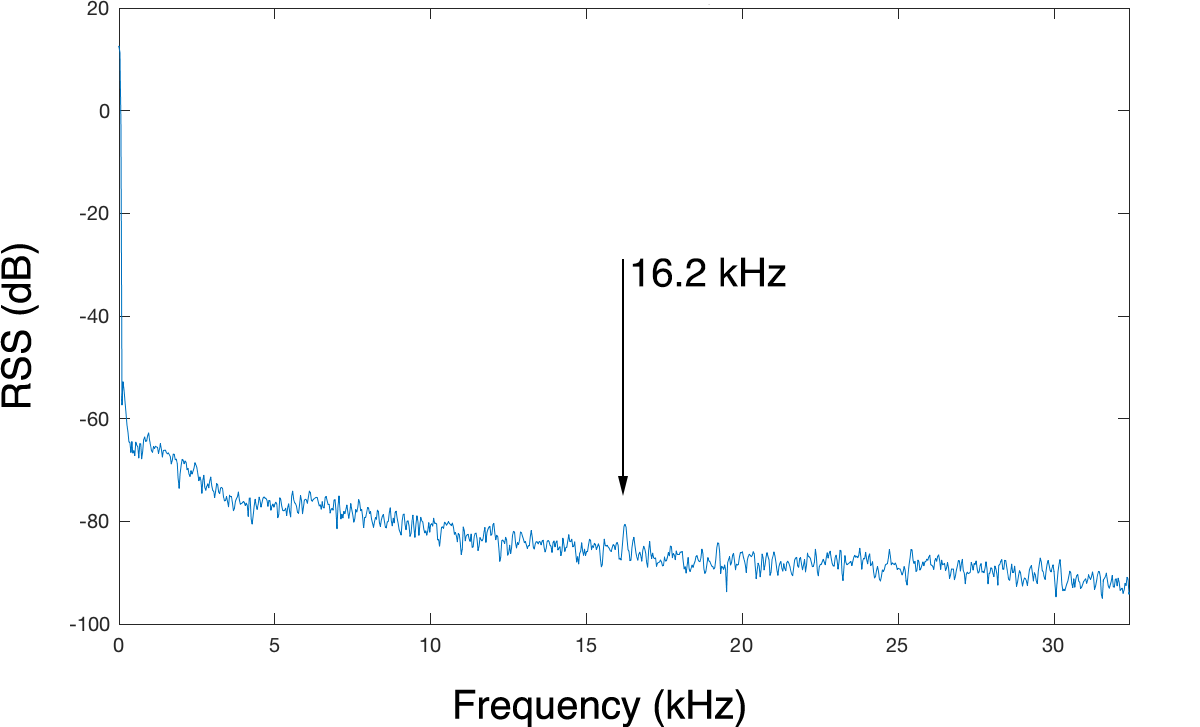
\includegraphics[width=1\linewidth]{figures/E/jpegs.png}
		\caption{JPEG compression emphasizing erroneous dominant frequency at 16.2 kHz}
	\end{subfigure}
	\begin{subfigure}{.5\textwidth}
		\centering
		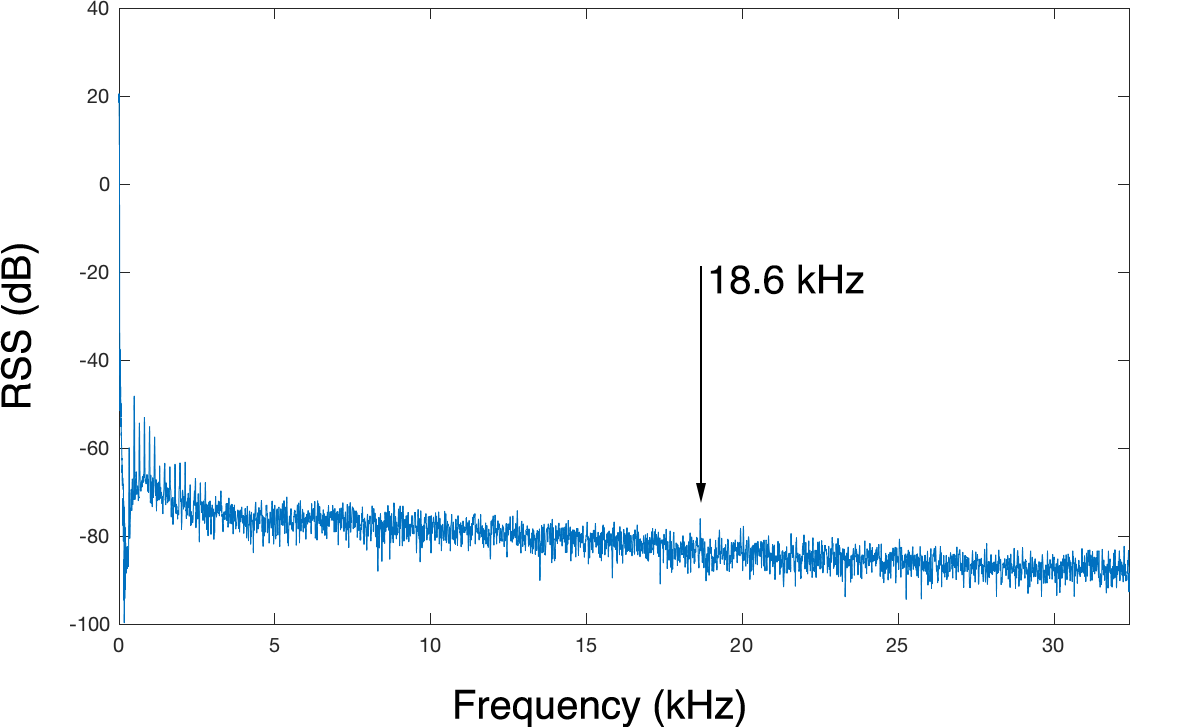
\includegraphics[width=1\linewidth]{figures/E/video.png}
		\caption{Video compression emphasizing unique frequency at 18.6 kHz and less dominant frequency at 16.2 kHz}
	\end{subfigure}
	\caption{JPEG compression vs. video compression for light \#2.}
	\label{fig:compressioncomparison}
\end{figure*}

We hypothesized in Section \ref{section:compression} that  JPEG compression removes the high intensity frequencies that we require for this research. To evaluate this hypothesis, we look at the differences in recorded frequencies between data formats captured from one light at an ISO value of 1201. We apply a Blackman filter to both sets of data and can see the resulting frequency spectrum in Fig. \ref{fig:compressioncomparison}. The data recorded from the video isolates a unique frequency around 18 kHz whereas the JPEG data only shows a dominant frequency at 16.2 kHz, a frequency we earlier regarded as common. Consequently, we believe that the unique, high frequency data is in fact removed by JPEG compression but retained in MP4 videos.

\subsection{Frequency Uniqueness}

\begin{figure*}[!h]
	\begin{subfigure}{.33\textwidth}
		\centering
		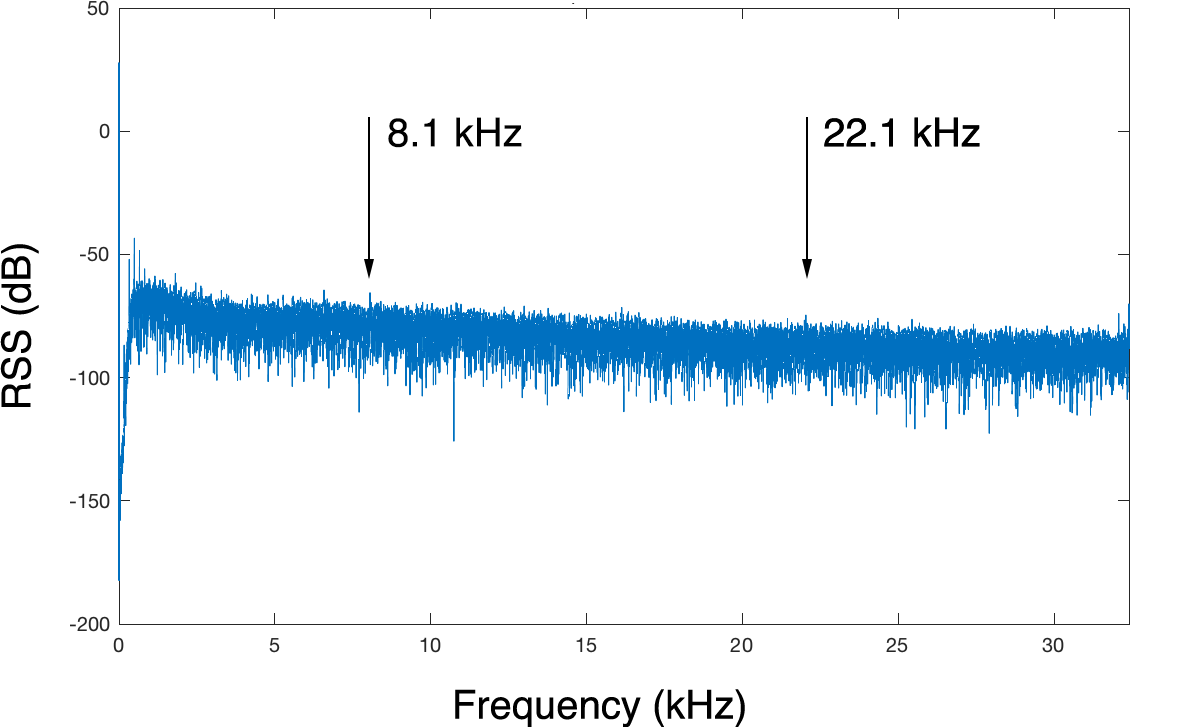
\includegraphics[width=1\linewidth]{figures/F/1.png}
		\caption{Light \#1 with peaks at 8.1 kHz, 22.1 kHz}
	\end{subfigure}
	\begin{subfigure}{.33\textwidth}
		\centering
		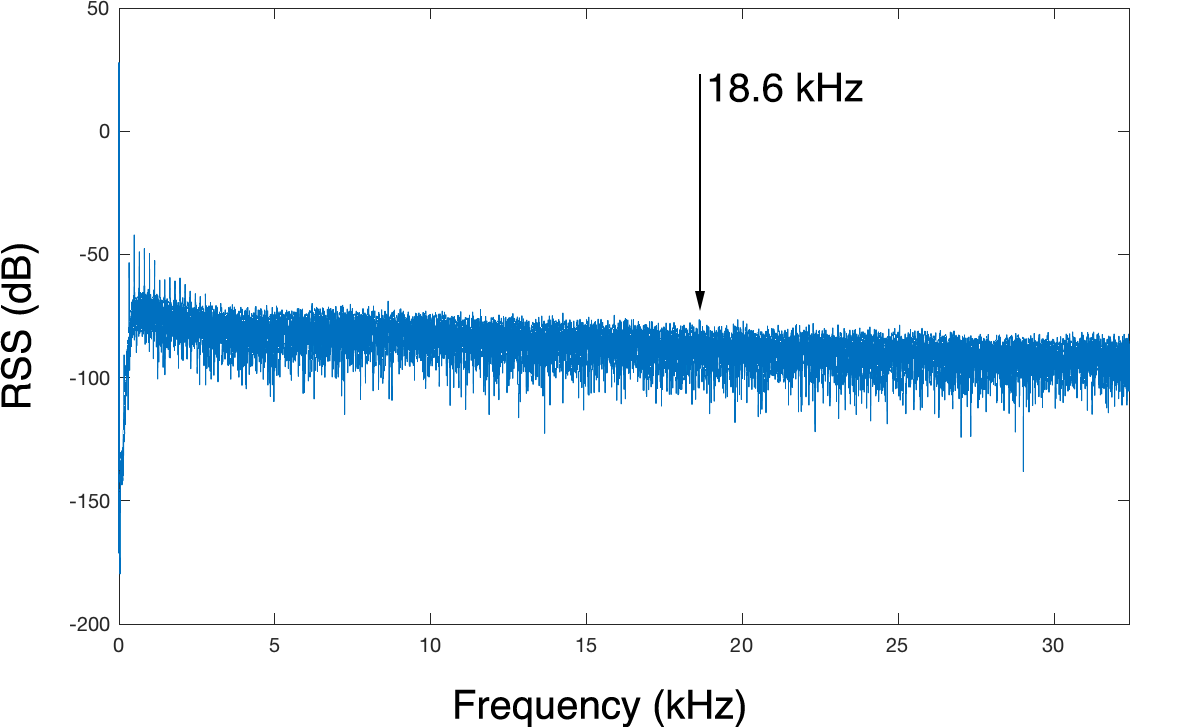
\includegraphics[width=1\linewidth]{figures/F/2.png}
		\caption{Light \#2 with peaks at 18.6 kHz}
	\end{subfigure}
	\begin{subfigure}{.33\textwidth}
		\centering
		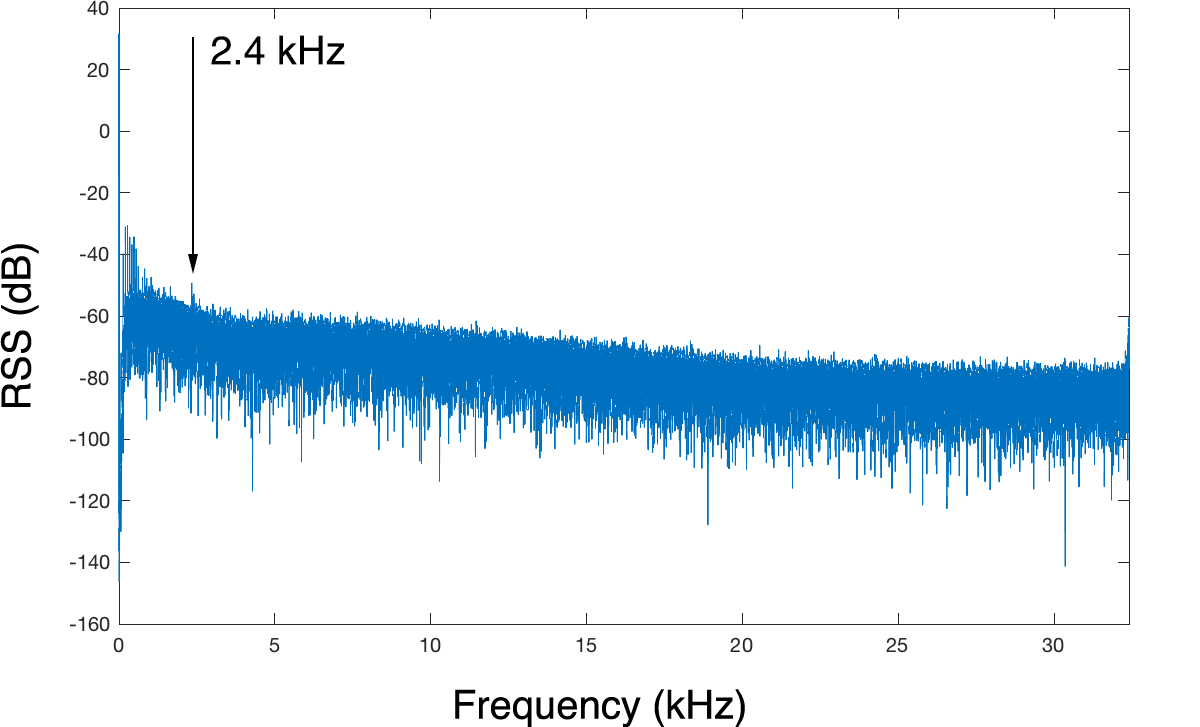
\includegraphics[width=1\linewidth]{figures/F/3.png}
		\caption{Light \#3 with peaks at 2.4 kHz}
	\end{subfigure}
	\caption{Unique frequency peaks across three different lights.}
	\label{fig:results}
\end{figure*}

Finally, we evaluate the effectiveness of identifying unmodified fluorescent lights simply by using video from a smartphone's front facing camera. We specifically analyze the resulting frequency spectrums obtained from our three experimental lights and emphasized the unique peaks in Fig. \ref{fig:results}. We find that light \#1 has two prominent peaks at 8.1 kHz and 22.1 kHz, light \#2 has a prominent peak at 18.6 kHz (which is made more visible after windowing in Fig. \ref{fig:compressioncomparison}.), and light \#3 has a prominent peak at 2.4 kHz.

Light \#3 has the strongest unique peak amidst the surrounding noise whereas light \#2 has the lowest. We believe that the SNR from light \#3 was significantly higher due to the shape of the light. Light \#1 and light \#2 were both U-shaped lights and the image processing algorithm acted over the two parallel sections independently. Light \#3, however, was one singular tube-shaped fluorescent light and consequently had a longer signal when run through the image processing algorithm. It appears, given Fig. \ref{fig:results}, that a longer signal in one frame results in a higher SNR.

Regardless of the differences in SNR, we have shown that there are unique frequency components between lights given no ambient light. Given a ground truth reading, we believe that filtering and proper windowing could be implemented to remove noisy data. Similarly, the image processing algorithm could potentially be modified to remove the erroneous peaks as defined earlier. We outline additional improvements in Section \ref{section:futurework}.

\section{Future Work}\label{section:futurework}

\subsection{Smartphone}

For sufficient image quality, typical smartphones shoot at $30$ frames per second. For the purpose of detecting high frequencies, however, this sampling rate is incomparable to the characteristic frequencies of fluorescent lights. While videos help in combating this issue by providing a large amount of samples over a given period of time, the sampling rate still remains too low. Although several phones are investigated in this paper and the smartphone with the best resolution was chosen, it would be worthwhile to search for a smartphone with an even greater camera resolution as increased camera quality would insure a more suitable sampling rate.

Furthermore, an alternative application to Open Camera should be developed that allows for more customization. While testing Open Camera on various smartphones, we found that not all camera2 API features were consistently functional. For example, when testing a Nexus 6, we were unable to manually modify the ISO level or shutter speed. Having full control over camera settings as well as more range with the shutter speed and ISO levels may grant better CF detection in the future.

LiTell was able to accurately identify unique frequency components because they utilized RAW images from the back-facing camera. As previously mentioned, the front-facing camera is only able to capture videos and JPEGs. In Section \ref{section:compression}, we define JPEGs as lossy images because they permanently eliminate high frequency components. While it would immensely help if the front-facing camera could also capture RAW images, the likelihood of that happening in the near future is low. Thus, other compression algorithms should also be examined, notably lossless compression techniques that retain more of the original pixel data.

\subsection{Experimental Set-Ups}

In \cite{zhang2016litell}, a database was created through fluorescent light fingerprinting, where the CF of each FL was sampled by a custom circuit and logged. In the future, having a measurement setup to record ground-truth CF values would allow for CF peak affirmation and also aid in the development of further noise suppression techniques. Similarly, the effects of ambient light and distance from camera-to-light should also be examined for real-world purposes.

\section{Conclusion}\label{section:conclusion}

In this paper, we explore the feasibility of using a conventional smartphone's front facing camera to distinguish between unmodified fluorescent lights. We capture videos on a Samsung Galaxy S8's front-facing camera and develop an image processing algorithm to extract aliased characteristic frequencies. Our evaluation shows that the front-facing camera has the ability to detect unique fluorescent light frequencies and offers significantly increased usability.

\section{Acknowledgement}\label{section:acnkowledgement}

This research was supported by the National Science Foundation (NSF) Research Experiences for Undergraduates (REU) program. We would like to thank all of the mentors and research fellows at the New York Institute of Technology who have provided their helpful insight and expertise that greatly assisted with our research.

We want to extend our thanks to the helpful graduate students, Mahmoud Saleh and Gopi Prasad, for their constant help over the program's duration. Similarly, we want to express our gratitude to the authors of \cite{zhang2016litell} for helping understand the complexities of their research.

This project is funded by National Science Foundation Grant No. CNS-1559652 and New York Institute of Technology.

\bibliography{bib} 
\bibliographystyle{ieeetr}

\end{document}
